\documentclass{beamer}

\usepackage[utf8]{inputenc}
\usepackage[T1]{fontenc}

\useinnertheme{default}
\useoutertheme[footline=authorinstitute,subsection=true]{miniframes}
%\useoutertheme{sidebar}
\usecolortheme{uconn}
\usefonttheme{uconn}

\setbeamercolor*{titlelike}{
    bg=uconn navy blue,
    fg=uconn white
}

\title[
    The 6th Report of Undergraduate Graduation Design
]{The 6th Report \\ of Undergraduate Graduation Design}
\subtitle{Research on laser interference \\ \& Something about programming $\dots$}
\author[Hao-si Li]{Hao-si Li}
\institute[Taiji Program]{The Department of Geophysics\\ Chang'an University}
\date{\today}

\newtheorem{remark}{Remark}

\begin{document}


\begin{frame}
\titlepage
\end{frame}


\begin{frame}{Table of contents}
\tableofcontents
\end{frame}


\section{Something about programming $\dots$}


\begin{frame}[fragile]{Concluding work of KBR}

In the last weeks, I complaint about the lack of the attitude data for GRACE FO. But it seemed the data package of LRI includes the essential information for calculating the cone angle of one satellite, AKA, \alert{yaw and pitch angle}. These two attitude angles are measured by laser interference.

\end{frame}


\begin{frame}[fragile]{The relationship between cone angle and attitude}

\begin{block}{Formula}
    \begin{equation}
        tan^2(cone \quad angle)=tan^2(yaw) + tan^2(pitch)
    \end{equation}
\end{block}

\begin{figure}
    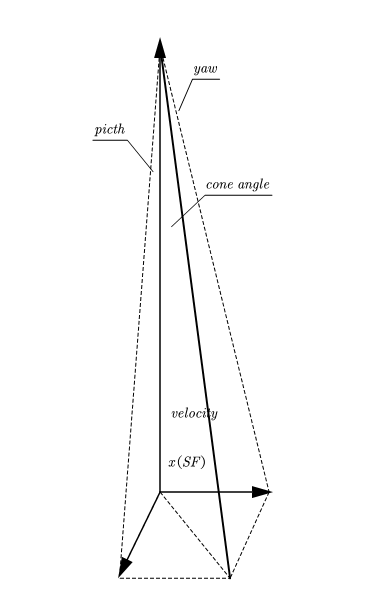
\includegraphics[height=2in]{images//cone_angle_relationship.png}
\end{figure}

\end{frame}


\begin{frame}{Error propagation formula}
\begin{block}{Formula}
    \begin{itemize}
        \item \begin{equation}
        \sigma _{n}^{2}\left( \delta T \right) =\frac{1}{1-P_n\left( cos\theta \right)}\frac{R_e}{GM}\left( \frac{r}{R_e} \right) ^{2n+1}\sigma _{n}^{2}\left( \delta \dot{\rho} \right) 
        \end{equation}
        \item \begin{equation}
            \sigma _{n}^{2}\left( \delta \dot{\rho} \right) =\sum_{n=0}^n{\left( \delta \bar{C}_{nm}^{2}+\delta \bar{S}_{nm}^{2} \right)}
        \end{equation}
    \end{itemize}
    
\end{block}

\end{frame}

\begin{frame}[fragile]{Some news}
    \begin{block}{News}
        \begin{itemize}
            \item \alert{Good news:} \\
            All the program work is finished $\dots$, including oscillator noise, system noise, multipath noise, error propagation and some plotting work.
            \item \alert{Bad news:} \begin{itemize}
                \item Not enough data, on the way solving.
                \item Last week, I found two IEEE articles about generating noise from prescribed PSD. These two methods are complicated and absolutely more accurate than my method which is generating the signal using filtering in the frequency domain regarding the given PSD as the filter. \alert{This problem must be solved!}
            \end{itemize}
        \end{itemize}
    \end{block}
    
\end{frame}


\begin{frame}[fragile]{Code review}
    
    Frankly speaking, I didn't finish enough work last week, so here it comes $\dots$
    
    \vfill
    
    In order to demonstrate explicitly, I am gonna switch to VSCODE $\dots$
\end{frame}


\section{Research on laser interference}
\label{sec:research}

\begin{frame}[fragile]{Reference}
    At first, I wanna read some articals or papers from Institute of mechanics, but nothing is found $\dots$.
    
    So I switch to read work from Huazhong University of science and technology and Harbin Institute of Technology.
    
    \begin{itemize}
        \item 
% TODO: \usepackage{graphicx} required
\begin{figure}
    \centering
    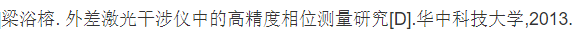
\includegraphics[width=0.7\linewidth]{images/liangyurong}
\end{figure}
        \item
% TODO: \usepackage{graphicx} required
\begin{figure}
    \centering
    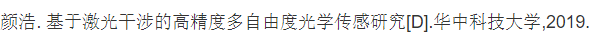
\includegraphics[width=0.7\linewidth]{images/yanhao}
\end{figure}
        \item
% TODO: \usepackage{graphicx} required
\begin{figure}
    \centering
    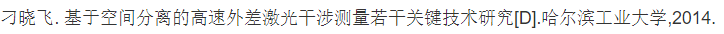
\includegraphics[width=0.7\linewidth]{images/diao}

\end{figure}

    \end{itemize}

Will ask Luo and Liu for some papers.
\end{frame}

\begin{frame}[fragile]{Difference frequency}
\begin{block}{The theorem of difference frequency}	
% TODO: \usepackage{graphicx} required
\begin{figure}
    \centering
    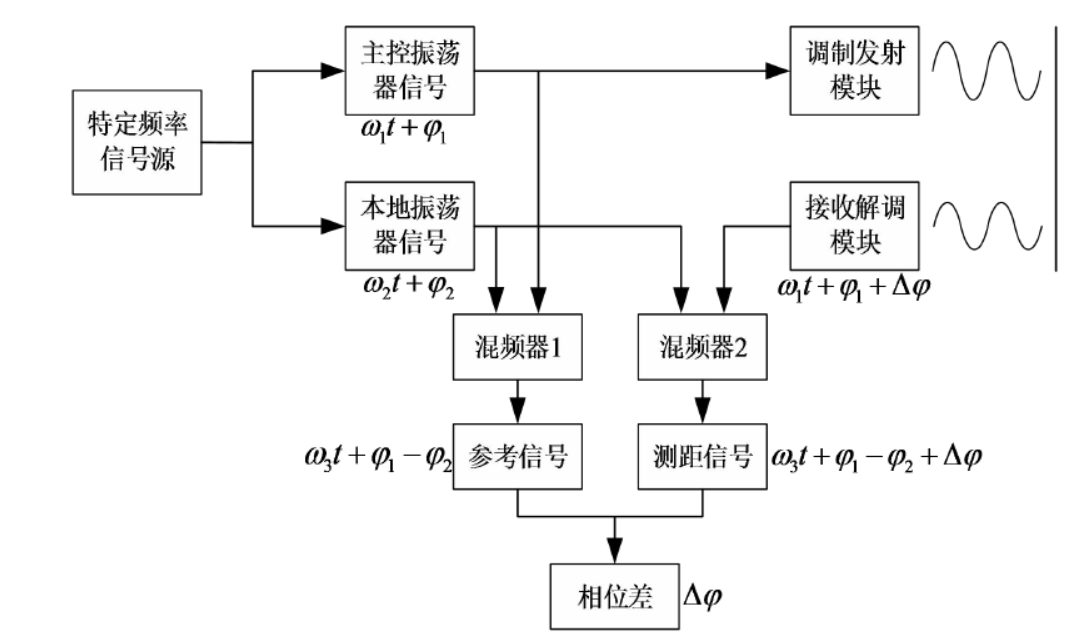
\includegraphics[width=0.7\linewidth]{images/chapin.png}
\end{figure}
\end{block}
\end{frame}

\begin{frame}[fragile]{Difference frequency}
    \begin{block}{Formula}
        \begin{itemize}
            \item Input 1: $y_1=A_1sin(2\pi f_1 t+\phi_1)$
            \item Input 2: $y_2=A_2sin(2\pi f_2 t+\phi_2)$
            \item Back: $S_1 = A_1^{'}sin(2\pi f_1 t + \phi_1 + \varDelta\phi)$
            \item the mixer = multiplier + low-pass filter
            \item $S_{ref} = y_1 \times y_2$
            \item $S_{dis} = y_1 \times S_1$
            \item the phase difference between $S_{ref}$ and $S_{dis}$ is what we concerned.
        \end{itemize}
    \end{block}
\end{frame}

\begin{frame}[fragile]{The principle of phasemetre AKA Two-way ranging}
    \begin{figure}
        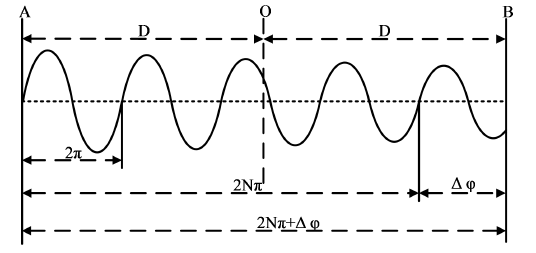
\includegraphics[width=0.5\linewidth]{images/two-way-ranging.png}
    \end{figure}

    \begin{block}{description}
        \begin{itemize}
            \item Two-way ranging: the one shot the laser is the same one to process the signal
            \item A: Shot point
            \item O: Reflection point
            \item B: Shot point, to exhibit explicitly
        \end{itemize}
    \end{block}
\end{frame}

\begin{frame}[fragile]{Two-way ranging}
    \begin{figure}
        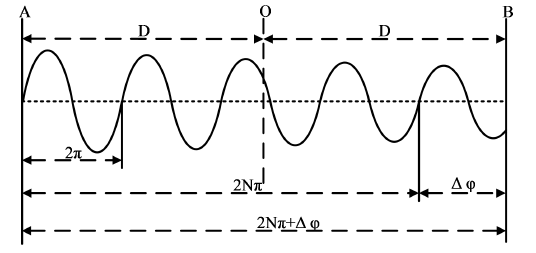
\includegraphics[width=0.5\linewidth]{images/two-way-ranging.png}
    \end{figure}
    
    \begin{block}{Principle}
        \begin{itemize}
            \item Transmitting singal: $S_1 = A_1 cos(\omega t_0 + \phi_0)$
            \item Received signal: $S_2 = A_2cos(cos\omega t_0 + \phi_0 + \phi)$
            \item No doubt, the loss of energy must exist
            \item Travelling time: $t = \frac{\phi}{2 \pi f}$
            \item Separation: $D = \frac{1}{2}ct = \frac{\lambda}{2}(N+\frac{\Delta \varphi}{2\phi})$
        \end{itemize}
    \end{block}
\end{frame}

\begin{frame}[fragile]{Two-way ranging}
    \begin{figure}
        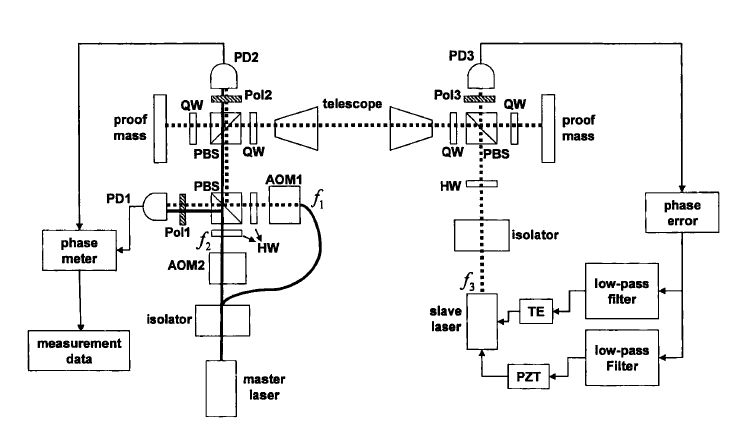
\includegraphics[width=0.8\linewidth]{images/liang.png}
        \caption{Schematic diagram}
    \end{figure}
\end{frame}

\begin{frame}[fragile]{Main error sources of laser interference}
    \begin{block}{Error sources}
        \begin{itemize}
            \item Unstable frequency of laser beamer Transmitter, \alert{but Luo said it is NOT important}
            \item Triple Mirror Assembly Pointing Jitter Coupling
            \item Unstablility because of temperature
            \item Additional Linear and Quadratic Pointing Jitter Coupling
            \item Noise from the phasemetre, can be neglected for now.
        \end{itemize}
    \end{block}
\end{frame}

\begin{frame}[fragile]{Frequency noise} 
    \begin{block}{Formula}
        According to the ground cavity performance test by JPL, the current best estimate of the
        ASD of the laser frequency noise for a satellite separation of 238km is:

        \begin{equation}
            \bar{\rho}_{LF}(f)=5 \times 10^{-9} \sqrt{1+(\frac{0.0182Hz}{f})^2} \frac{m}{\sqrt{Hz}}
        \end{equation}
    \end{block}
\end{frame}

\begin{frame}[fragile]{ASD diagram}
    \begin{figure}
        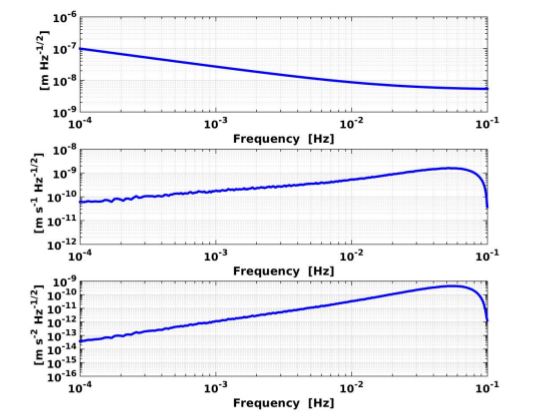
\includegraphics[width=0.8\linewidth]{images/freq.png}
    \end{figure}
\end{frame}

\begin{frame}[fragile]{Problem coming $\dots$}
    This is another problem about generating noise from a prescribed ASD/PSD.

    The only solution is filtering for now $\dots$

    The theories in those two papers will certainly be useful in the future, so one of the tasks in the graduate stage is to solve this problem.
    
\end{frame}


\section{Thanks}


\begin{frame}
\begin{Huge}
    \centering
    Thank you!
\end{Huge}
\end{frame}


\end{document}